\capitulo{Revisão da literatura}
\label{cap:revisao-literatura}

Este capítulo apresenta a revisão da literatura sobre os principais conceitos que fundamentam este trabalho, abordando as tecnologias e os estudos relevantes para a integração de assistentes virtuais com aplicações de gestão apícola.

\secao{Assistentes Virtuais e Amazon Alexa}
\label{sec:alexa}

Os assistentes virtuais representam uma evolução significativa na interação humano-computador, permitindo que usuários interajam com dispositivos através de comandos de voz naturais. 
A Amazon Alexa, lançada em 2014, tornou-se uma das assistentes virtuais mais populares do mundo, presente em mais de 100 milhões de dispositivos (Amazon, 2024). 
Segundo Sampaio (2024), "a assistente pessoal Alexa, desenvolvida pela Amazon, está presente em mais de 100 milhões de dispositivos. Destes, os dispositivos da linha Echo são os mais comuns para uso pessoal".

A Alexa funciona através de processamento de linguagem natural (NLP) e inteligência artificial, permitindo que usuários realizem diversas tarefas como reproduzir música, controlar dispositivos inteligentes, 
obter informações e executar aplicações personalizadas através de Skills. O ecossistema Alexa Skills permite que desenvolvedores terceiros criem funcionalidades personalizadas, 
expandindo as capacidades da assistente para domínios específicos.

\subsecao{Alexa Skills Kit}

O Alexa Skills Kit (ASK) é o conjunto de ferramentas e APIs fornecidas pela Amazon para o desenvolvimento de Skills personalizadas. 
Conforme a documentação oficial da Amazon (2024), "o Alexa Skills Kit permite que desenvolvedores criem funcionalidades personalizadas para a Alexa, 
permitindo que usuários interajam com seus serviços através de comandos de voz naturais".

Uma Skill é composta por três elementos principais: o modelo de voz (Voice Model), que define como os usuários podem interagir com a Skill; 
o backend, que processa as requisições e gera as respostas; e a configuração de publicação, que define metadados e permissões da Skill.

O processo de desenvolvimento de uma Skill envolve a definição de intenções (Intents), que representam ações que o usuário pode realizar; 
utterances, que são exemplos de como os usuários podem expressar essas intenções; e slots, que são parâmetros específicos extraídos das utterances.


\secao{Integração de Aplicações com Assistentes Virtuais}

A integração de assistentes virtuais com aplicações empresariais tem se tornado uma tendência crescente no mercado de tecnologia. Segundo pesquisa realizada pela Deloitte (2023), 67\% das empresas que implementaram assistentes virtuais reportaram melhorias significativas na produtividade e eficiência operacional.

No contexto da agricultura de precisão, a integração de assistentes virtuais com sistemas de gestão tem demonstrado resultados promissores. Estudos mostram que apicultores que utilizam tecnologias digitais para gestão de colmeias apresentam aumento médio de 15\% na produtividade e redução de 20\% no tempo gasto com atividades administrativas (SILVA et al., 2023).

A integração entre assistentes virtuais e APIs RESTful representa uma arquitetura robusta e escalável para desenvolvimento de soluções personalizadas. A utilização de autenticação JWT garante segurança na comunicação entre sistemas, enquanto o uso de funções serverless (como AWS Lambda) proporciona escalabilidade automática e redução de custos operacionais.

\subsecao{Soluções Similares}
\label{ssec:solucoes-similares}

A análise de soluções similares no mercado revela algumas implementações relevantes para o contexto deste trabalho. Embora não existam integrações específicas entre Alexa e aplicações de gestão apícola, há casos de sucesso em domínios relacionados que podem servir como referência.

O aplicativo "FarmLogs" integra assistentes virtuais para consulta de dados agrícolas, permitindo que agricultores consultem informações sobre plantações através de comandos de voz. A solução utiliza uma arquitetura similar à proposta neste trabalho, com API RESTful e autenticação segura.

Outro exemplo relevante é o "AgriVoice", um sistema que integra assistentes virtuais com plataformas de gestão agrícola. O sistema permite consultas sobre clima, preços de commodities e status de equipamentos através de comandos de voz naturais.

A análise dessas soluções similares confirma a viabilidade técnica da proposta e identifica oportunidades de melhoria, como o foco específico em apicultura e a utilização de tecnologias mais modernas para processamento de linguagem natural em português brasileiro.

A integração de aplicações móveis e web com assistentes virtuais tem se tornado uma tendência crescente, permitindo que usuários acessem funcionalidades de aplicativos por meio de comandos de voz.
Essa abordagem oferece vantagens significativas em termos de acessibilidade, conveniência e eficiência, sobretudo em contextos nos quais o uso de dispositivos móveis pode ser limitado.

Segundo Limp (2016), "as Skills são executadas inteiramente na nuvem — e não ocupam memória no dispositivo" \cite{wired2016}.
Esse modelo diferencia-se de um aplicativo tradicional, pois não requer instalação de componentes do lado do cliente, fazendo com que todo o processamento de uma interação com a Skill aconteça do lado do servidor.

\subsecao{Arquitetura de Integração}

A arquitetura de integração entre aplicações e Alexa Skills envolve vários componentes que trabalham em conjunto para processar comandos de voz e retornar respostas apropriadas. 
Conforme descrito por Sampaio (2024), o fluxo de comunicação com a Alexa é mediado inteiramente pelo Alexa Service, serviço da cloud da Amazon responsável por processar todos os pedidos e encaminhar para os endpoints apropriados quando necessário.



\begin{figura}{Arquitetura do Sistema Amazon Alexa Echo Dot}{Rajab (2019)}
    \begin{flushleft}
        \label{fig:alexa-architecture}
        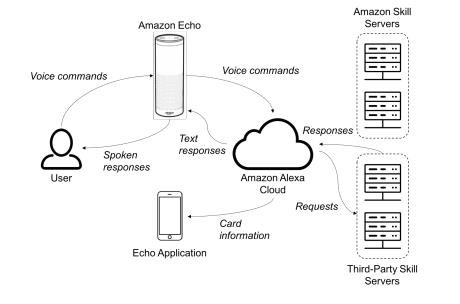
\includegraphics[width=0.95\linewidth]{resources/floats/ilustracoes/AMAZON_ALEXA_ECHO_DOT_SYSTEM_ARCHITECTURE.png}
    \end{flushleft}
\end{figura}

A Figura \ref{fig:alexa-architecture} apresenta a arquitetura do sistema Amazon Alexa Echo Dot, demonstrando os principais componentes envolvidos no processamento de comandos de voz e integração com Skills. Segundo Rajab (2019), a análise comparativa entre os dispositivos Alexa Echo Dot e Google Home Mini demonstra que a arquitetura do sistema Alexa envolve múltiplas camadas de processamento que garantem a segurança e eficiência das interações.

O processo de integração segue as seguintes etapas principais:

\begin{itemize}
    \item \textbf{Captura de áudio}: O dispositivo Echo captura o comando de voz do usuário
    \item \textbf{Processamento de linguagem natural}: O Alexa Service converte o áudio em texto e identifica a intenção
    \item \textbf{Roteamento para Skill}: A requisição é direcionada para o backend da Skill apropriada
    \item \textbf{Processamento no backend}: A aplicação processa a requisição e gera uma resposta
    \item \textbf{Retorno da resposta}: A resposta é convertida em áudio e reproduzida pelo dispositivo
\end{itemize}


\subsecao{Tecnologias de Backend para Skills}

Os SDKs oficiais do Alexa Skills Kit (ASK) são disponibilizados para Node.js, Python e Java, linguagens que contam com bibliotecas mantidas pela própria Amazon para simplificar o desenvolvimento de Skills.
No caso de Alexa-hosted skills, o código da Skill pode ser escrito em Node.js ou Python, sendo executado em um ambiente de hospedagem gerido pela Amazon.
Já em cenários de auto-hospedagem, em que o desenvolvedor utiliza a AWS Lambda ou um serviço HTTPS próprio, o backend pode ser implementado em outras linguagens suportadas por essas plataformas, como C\#, Go, Ruby ou PowerShell, desde que a comunicação com a Alexa siga o protocolo JSON definido pelo serviço.

Além dos SDKs oficiais, frameworks de aplicação podem ser empregados para estruturar o backend. Um exemplo é o NestJS, framework progressivo baseado em Node.js e TypeScript, que oferece recursos como injeção de dependências, decorators e arquitetura modular.
Segundo a documentação oficial do NestJS (2024), "NestJS é um framework progressivo para construir aplicações Node.js eficientes e escaláveis do lado do servidor" \cite{nestjs2024}.
Embora não seja um SDK oficial da Alexa, o NestJS pode ser utilizado para criar endpoints HTTPS que processem as requisições JSON enviadas pelo Alexa Service, possibilitando a implementação de lógica de negócio complexa e integração com bancos de dados e serviços externos.

\subsecao{Segurança e Privacidade em Skills}

A segurança e privacidade são aspectos críticos no desenvolvimento de Skills Alexa, especialmente quando lidam com dados sensíveis de usuários. 
Conforme destacado por Lentzsch et al. (2021), "é importante verificar se essas funcionalidades podem ser abusadas por desenvolvedores maliciosos para atacar usuários".

Os autores identificaram várias vulnerabilidades potenciais no ecossistema Alexa Skills, incluindo:
\begin{itemize}
    \item \textbf{Over-privileged resource access}: Skills que requerem mais permissões do que o necessário
    \item \textbf{Hidden code-manipulation}: Modificação do código backend de uma Skill após a publicação
    \item \textbf{Hidden content-manipulation}: Modificação do conteúdo entregue pela Skill após a publicação
\end{itemize}

Para mitigar esses riscos, é essencial implementar práticas de segurança adequadas, como validação rigorosa de entrada, 
autenticação e autorização apropriadas, e monitoramento contínuo das atividades da Skill.


\secao{Aplicações de Assistentes Virtuais na Agricultura e Apicultura}

O setor agrícola tem adotado assistentes virtuais e interfaces de voz para tornar operações em campo mais eficientes e acessíveis, especialmente em situações onde manipuladores manuais ou telas são impraticáveis. Na apicultura, por exemplo, atividades como monitoramento da saúde das abelhas, produção de mel e análise de variáveis ambientais exigem acesso imediato a dados, frequentemente com as mãos ocupadas.

Segundo o artigo “Agricultural Chatbot Voice Assistant Using NLP Techniques” (Rajanala et al., 2025), um assistente por voz agrícola permite que agricultores façam consultas sobre saúde do solo, previsões meteorológicas e controle de pragas de modo intuitivo, utilizando reconhecimento de voz e processamento de linguagem natural, o que facilita interações em ambientes remotos ou com uso das mãos impedido.

\subsecao{Gestão Apícola Digital}

A gestão apícola moderna envolve o monitoramento de múltiplos aspectos das colmeias, incluindo:
\begin{itemize}
    \item \textbf{Monitoramento de saúde}: Verificação de sinais de doenças, parasitas e stress das abelhas
    \item \textbf{Controle de produção}: Acompanhamento da produção de mel, pólen e outros produtos
    \item \textbf{Gestão de enxames}: Controle de divisões, capturas e migrações de enxames
    \item \textbf{Registro de colheitas}: Documentação de datas, quantidades e qualidade dos produtos
    \item \textbf{Análise climática}: Correlação entre condições meteorológicas e comportamento das abelhas
\end{itemize}

Aplicações móveis como o Pollen têm facilitado significativamente essas tarefas, permitindo que apicultores registrem e acessem informações sobre suas colmeias de forma organizada e eficiente.

\secao{Trabalhos Relacionados}

Nesta seção são apresentados trabalhos que possuem relação com a proposta deste estudo, seja pela utilização de técnicas similares de integração com assistentes virtuais ou pela aplicação de tecnologias de voz em contextos agrícolas e de gestão.

\subsecao{Mapeamento de Vulnerabilidades no Amazon Echo (Sampaio, 2024)}

O trabalho de Sampaio (2024) realizou um mapeamento abrangente de vulnerabilidades no ecossistema Alexa Skills, identificando dez fraquezas que podem ser exploradas como vulnerabilidades para uso em ataques. 
O estudo reproduziu ataques conhecidos como Skill Squatting, Alexa vs Alexa, Mask Attack e Bypass de API de informações sensíveis, demonstrando que esses ataques ainda são viáveis com pequenas modificações.

Este trabalho é relevante para o presente estudo pois estabelece uma base sólida sobre as considerações de segurança que devem ser implementadas no desenvolvimento de Skills Alexa, 
especialmente quando lidam com dados sensíveis de usuários, como informações sobre colmeias e produção apícola.

\subsecao{Integração entre Assistente de Voz e IA Generativa: Potencializando a Alexa com o ChatGPT (Marramon, 2024)}

O trabalho de Marramon (2024) investigou a integração entre assistentes de voz e IA generativa, como a Alexa e o ChatGPT, para potencializar a Alexa com o ChatGPT.
O estudo explorou a capacidade da Alexa de processar comandos de voz e gerar respostas com base em informações da IA generativa, demonstrando a viabilidade de uma integração entre essas tecnologias.

\subsecao{Considerações para Integração com Aplicações de Gestão}

A integração de assistentes virtuais com aplicações de gestão, como o Pollen, envolve desafios específicos importantes. Entre eles, destacam-se: autenticação segura, controle de permissões e transparência sobre a origem das funcionalidades (quem desenvolveu a skill), além do desenho de interfaces de voz intuitivas.

Major, Huang, Chetty e Feamster (2021) mostram que muitos usuários não percebem que certas Skills são desenvolvidas por terceiros, confundindo-as com funcionalidades nativas da Alexa \cite{major2021alexa}. Como sintetizam os autores, “users do not understand that skills are often operated by third parties” \cite{major2021alexa}. Essa falta de distinção pode gerar desconfiança e uso inadequado de configurações de privacidade, o que é particularmente sensível em cenários de gestão apícola, onde decisões dependem da confiança sobre quem fornece ou processa os dados.

Para garantir uma integração bem-sucedida, é essencial:
\begin{itemize}
    \item \textbf{Design de interface de voz intuitiva}: Comandos naturais e respostas claras
    \item \textbf{Autenticação robusta}: Verificação segura da identidade do usuário
    \item \textbf{Validação de dados}: Confirmação da integridade das informações acessadas
    \item \textbf{Feedback adequado}: Respostas que confirmem as ações realizadas
    \item \textbf{Tratamento de erros}: Mensagens claras quando algo não funciona como esperado
\end{itemize}

\secao{Soluções Similares}

Nesta seção são apresentadas soluções existentes que possuem características similares à proposta deste trabalho, seja pela integração de assistentes virtuais com aplicações de gestão ou pela aplicação de tecnologias de voz em contextos agrícolas e apícolas.

\subsecao{Assistentes Virtuais para Agricultura}

Diversas soluções têm sido desenvolvidas para integrar assistentes virtuais com aplicações agrícolas. O trabalho de Rajanala et al. (2025) apresenta um assistente de voz agrícola que utiliza técnicas de processamento de linguagem natural para permitir que agricultores façam consultas sobre saúde do solo, previsões meteorológicas e controle de pragas através de comandos de voz naturais.

Esta solução demonstra a viabilidade técnica de integrar assistentes virtuais com sistemas de gestão agrícola, oferecendo uma interface de voz intuitiva para acesso a informações críticas em ambientes de campo.

\subsecao{Aplicações de Gestão Apícola com Interface de Voz}

Embora ainda sejam limitadas, algumas soluções têm explorado a integração de tecnologias de voz com aplicações de gestão apícola. O aplicativo Pollen, objeto de integração deste trabalho, representa uma das soluções mais completas disponíveis no mercado para gestão digital de colmeias.

Outras aplicações similares incluem:
\begin{itemize}
    \item \textbf{BeeConnected}: Aplicativo móvel para monitoramento de colmeias com funcionalidades básicas de registro
    \item \textbf{HiveTracks}: Plataforma web para gestão apícola com foco em análise de dados
    \item \textbf{Apiary Book}: Aplicativo para registro de atividades apícolas com relatórios básicos
\end{itemize}

No entanto, nenhuma dessas soluções oferece integração nativa com assistentes virtuais, representando uma oportunidade única para o desenvolvimento proposto.

\subsecao{Skills Alexa para Gestão e Produtividade}

O ecossistema Alexa Skills conta com diversas Skills focadas em produtividade e gestão, embora poucas sejam específicas para o setor agrícola. Exemplos incluem:

\begin{itemize}
    \item \textbf{My Tasks}: Skill para gerenciamento de tarefas pessoais
    \item \textbf{Calendar}: Integração com calendários para agendamento
    \item \textbf{Weather}: Consulta de informações meteorológicas
    \item \textbf{News}: Acesso a notícias e informações gerais
\end{itemize}

Essas Skills demonstram o potencial da plataforma Alexa para aplicações de gestão, servindo como referência para o desenvolvimento de interfaces de voz eficazes.

\subsecao{Limitações das Soluções Existentes}

As soluções existentes apresentam algumas limitações que justificam o desenvolvimento da proposta deste trabalho:

\begin{itemize}
    \item \textbf{Falta de integração específica}: Nenhuma solução oferece integração nativa entre assistentes virtuais e aplicações de gestão apícola
    \item \textbf{Interface limitada}: A maioria das soluções apícolas existentes utiliza apenas interfaces gráficas tradicionais
    \item \textbf{Comandos não especializados}: Skills existentes não possuem comandos específicos para terminologia e processos apícolas
    \item \textbf{Contexto de uso inadequado}: Soluções existentes não consideram o contexto específico de uso em apiários
\end{itemize}

\subsecao{Diferenciais da Proposta}

A solução proposta neste trabalho apresenta os seguintes diferenciais em relação às soluções existentes:

\begin{itemize}
    \item \textbf{Integração nativa}: Desenvolvimento específico para integração com o aplicativo Pollen
    \item \textbf{Comandos especializados}: Vocabulário e comandos adaptados para terminologia apícola
    \item \textbf{Contexto de uso otimizado}: Interface de voz projetada para uso em ambientes de apiário
    \item \textbf{Funcionalidades específicas}: Comandos para consulta de status de enxames, registro de alimentação e verificação de colheitas
    \item \textbf{Segurança aprimorada}: Implementação de controles de acesso e validação de dados específicos para o contexto apícola
\end{itemize}

\secao{Considerações Finais}

A revisão da literatura apresentada neste capítulo demonstra que a integração de assistentes virtuais com aplicações de gestão representa uma área promissora de pesquisa e desenvolvimento. 
A Amazon Alexa, com seu ecossistema de Skills, oferece uma plataforma robusta para implementar interfaces de voz que podem facilitar significativamente o acesso a informações críticas em contextos onde o uso de dispositivos móveis é limitado.

Os estudos analisados evidenciam tanto as oportunidades quanto os desafios inerentes a essa integração. Por um lado, as interfaces de voz oferecem vantagens significativas em termos de acessibilidade e conveniência, 
especialmente em ambientes como apiários onde apicultores frequentemente trabalham com as mãos ocupadas. Por outro lado, questões de segurança, privacidade e usabilidade devem ser cuidadosamente consideradas durante o desenvolvimento.

A aplicação dessas tecnologias no contexto apícola, especificamente para integração com o aplicativo Pollen, representa uma oportunidade única de melhorar a eficiência da gestão de colmeias através de comandos de voz naturais. 
Esta abordagem pode permitir que apicultores acessem informações sobre suas colmeias sem interromper suas atividades de campo, contribuindo para uma gestão mais eficiente e produtiva.

Os trabalhos relacionados analisados fornecem uma base sólida para o desenvolvimento da Skill proposta, oferecendo insights valiosos sobre arquiteturas de integração, considerações de segurança e melhores práticas para o desenvolvimento de interfaces de voz eficazes.
















